\documentclass[finnish]{tktltiki2}

% --- General packages ---

\usepackage[utf8]{inputenc}
\usepackage[T1]{fontenc}
\usepackage{lmodern}
\usepackage{microtype}
\usepackage{amsfonts,amsmath,amssymb,amsthm,booktabs,color,graphicx}
\usepackage[pdftex,hidelinks]{hyperref}
% Automatically set the PDF metadata fields
\makeatletter
\AtBeginDocument{\hypersetup{pdftitle = {\@title}, pdfauthor = {\@author}}}
\makeatother

% --- Language-related settings ---
%
% these should be modified according to your language

% babelbib for non-english bibliography using bibtex
\usepackage[fixlanguage]{babelbib}
\selectbiblanguage{finnish}

% add bibliography to the table of contents
\usepackage[nottoc]{tocbibind}
% tocbibind renames the bibliography, use the following to change it back
\settocbibname{Lähteet}

% --- Theorem environment definitions ---

\newtheorem{lau}{Lause}
\newtheorem{lem}[lau]{Lemma}
\newtheorem{kor}[lau]{Korollaari}

\theoremstyle{definition}
\newtheorem{maar}[lau]{Määritelmä}
\newtheorem{ong}{Ongelma}
\newtheorem{alg}[lau]{Algoritmi}
\newtheorem{esim}[lau]{Esimerkki}

\theoremstyle{remark}
\newtheorem*{huom}{Huomautus}

\def\figureautorefname{kuva}

% --- tktltiki2 options ---
%
% The following commands define the information used to generate title and
% abstract pages. The following entries should be always specified:

\title{Samanaikaisuus verkkopalvelinsovelluksessa}
\author{Vili Lipo}
\date{\today}
\level{Kandidaatin tutkielma}
\abstract{Tässä tutkielmassa vertaillaan verkkopalvelimien suunnittelumalleja
  ja niiden suorituskykyä. Verkkopalvelin on ohjelma, joka vastaa useiden asiakkaiden pyyntöihin
  verkkosivuilla tai verkkosovelluksissa. Pyyntöihin vastaamiseen
  voi liittyä laskentaa, tietokantaoperaatioita tai muita toimenpiteitä.

Vertailuun valittiin tapahtumaohjattu Reactor-malli, SEDA-malli ja säiereservimalli}

% The following can be used to specify keywords and classification of the paper:

\keywords{palvelin, tapahtumaohjattu, samanaikaisuus}

% classification according to ACM Computing Classification System (http://www.acm.org/about/class/)
% This is probably mostly relevant for computer scientists
% uncomment the following; contents of \classification will be printed under the abstract with a title
% "ACM Computing Classification System (CCS):"
\classification{Software and its engineering $\rightarrow$ Software organization and properties
$\rightarrow$ Software system structures $\rightarrow$ Distributed systems organizing principles}

% If the automatic page number counting is not working as desired in your case,
% uncomment the following to manually set the number of pages displayed in the abstract page:
%
% \numberofpagesinformation{16 sivua + 10 sivua liitteissä}
%
% If you are not a computer scientist, you will want to uncomment the following by hand and specify
% your department, faculty and subject by hand:
%
% \faculty{Matemaattis-luonnontieteellinen}
% \department{Tietojenkäsittelytieteen laitos}
% \subject{Tietojenkäsittelytiede}
%
\begin{document}
\frontmatter      % roman page numbering for front matter

\maketitle        % title page
\makeabstract     % abstract page

\tableofcontents  % table of contents

% --- Main matter ---

\mainmatter       % clear page, start arabic page numbering

\section{Johdanto}
Verkkopalvelinsovelluksien suorituskyky vaikuttaa vahvasti
Internetin välityksellä käytettävien palveluiden käyttökokemukseen ja toimivuuteen.
Verkkopalvelimien taakat ovat vaihtelevia, ja tästä johtuen
yleispätevän verkkopalvelimen tulisi skaalautua saatavilla oleviin resursseihin.
Jos verkkopalvelimen käyttötarkoitus ei ole suorittaa laskennallisesti raskaista
tehtäviä, sen
kriittisimmät resurssit ovat I/O-resurssit.

Verkkopalvelimen tehokkuuteen ja skaalautumiseen vaikuttaa olennaisesti
sen samanaikaistamismalli. Tässä
tutkielmassa vertaillaan eri suunnittelumalleja palvelimen toimintojen samanaikaistamiseen.

Samaikaisessa ohjelmassa ohjelman osat ovat näennäisesti samaan
aikaan suorituksessa, mutta todellisuudessa ne suoritetaan peräkkäin.
Käyttöjärjestelmä jakaa suoritusaikaa ohjelman eri osille,
ja vuorottelemalla antaa vaikutelman samanaikaisuudesta.

Rinnakkaisuudella tarkoitetaan tietojenkäsittelytieteessä useiden
eri operaatioiden suorittamista järjestelmässä samaan aikaan useilla suorittimilla.
Rinnakkaisuutta voi
ajatella samanaikasuuden seuraavana asteena. Kun suorittimia
on useita, käyttöjärjestelmä pystyy aikatauluttamaan toimintoja
rinnakkain ja näin kaksi ohjelman osaa on todellisesti
samaan aikaan suorituksessa.

Verkkopalvelimen samanaikaistamismalli on osa palvelinsovellusta,
joka on mielekästä toteuttaa moduulina tai kirjastona.
Näin palvelimen sovelluslogiikka voidaan irrottaa rinnakkaisuutta
käsittelevästä logiikasta ja käyttää uudelleen toisissa projekteissa.
Tavoitteena on selvittää mikä suunnittelumalli edistää
parhaiten verkkopalvelinsovelluksen suorituskykyä ja
kehitystyötä.

Vertailussa perehdytään Reactor-malliin\cite{schmidt_reactor:_1995} ja sen jatkokehityksiin
kuten Proactor-malliin~\cite{pyarali_proactor_1997}, säiereservimalliin (threadpool-model)
ja SEDA-malliin.
Vertailun keskeisimmät kriteerit ovat suorituskyky, vakaus, ja
sovelluslogiikan kehittämiseen liittyvät haasteet.

Verkkopalvelinsovelluksen suorituskyky ja skaalautuvuus
määrittävät palvelun laadun raskaan kuormituksen tilanteissa.
Poikkeus-ja virhetilanteet vaikuttavat hyvin negatiivisesti
palvelun laatuun. Jos poikkeustilanne johtaa
palvelun kaatuamiseen, voivat seuraamukset olla vakavat
palvelun ylläpitäjän ja asiakkaiden kannalta.
Palvelimen suunnittelumalli voi vaikuttaa 
sovelluskohtaisen logiikan kehittämiseen.
Jos malli tekee kehitystyöstä hyvin, haastavaa
nousee kehitystyön kustannukset.
Suunnittelumallin tulisikin edistää
samanaikaisuutta ja rinnakkaisuutta vaikeuttamatta
sovelluslogiikan kehitystä suuremmin.

Vertailun perusteella voidaan todeta että,
% TODO: Kappaleen hurjiin väitteisiin lähde
yksinkertaisuudestaan huolimatta tehokkailla asynkronisilla
kutsuilla varustettu Reactor-mallinen verkkopalvelinsovellus
kykenee vastaamaan suurenkin palvelun tarpeisiin, jos palvelun
pullonkaula on I/O-operaatiot.
Proactor-mallilla voidaan tarjota kehittäjille edistyneempiä työkaluja
asynkronisten operaatioiden hallintaan.

Tarvittaessa järjestelmän voi laajentaa moniprosessimallia noudattavaksi,
jos tapahtumaohjatun järjestelmän skaalautuvuus ei muuten riitä.

Säiereservimallin on hyvä vaihtoehto, jos palvelimen
toimintaan liittyy enemmän laskentaa ja sen tehokkuus ei ole I/O-sidonnainen.
Laskennallisesti raskaaseen palvelimeen voidaan myös soveltaa SEDA-mallia~\cite{welsh_seda_2001}.
Siinä pyyntöjen käsittely jaetaan eri tasoille ja tasojen käsíttelyyn
hyödynnetään säiereservejä.

Luvussa~\ref{vps} kerrotaan taustatietota asiakas-palvelin-mallista, palvelinympäristöstä
ja rinnakkaisuudesta.
Luvussa~\ref{sec:SM} verkkopalvelimien suunnittelumalleja. Luvussa~\ref{sec:vertailu}
malleja vertaillaan ja analysoidaan. Luvussa~\ref{sec:yhteenveto} on yhteenveto aiheesta.

\section{Verkkopalvelinsovellus}\label{vps}
Verkkopalvelinsovellus on osa internetsivuston tai palvelun tarjoavaa
asiakas-palvelin-mallin toteutusta. 
Sen tehtävä on vastata Internet-
sivuston tai palvelun toteuttamiseen
liittyviin pyyntöihin eli lähettämään tietyn HTTP-pyynnön
perusteella oikea HTML-tiedosto, tekstimuotoinen datatiedosto~\cite{Berners-Lee_1994}
,tai kuvatiedosto.

Tässä luvussa kerrataan
asiakas-palvelin-malli ja rinnakkaisuuden keskeiset käsitteet.
Sen jälkeen käydään läpi eri malleja rinnakkaisuuden edistämiseen
verkkopalvelimissa. Malleista tutkitaan erityisesti miten I/O-operaatioita
suoritetaan samanaikaisesti. Mallien toimintaa havainnollistetaan
esittämällä esimerkkejä asiakkaan pyynnön käsittelystä mallin
toteuttavassa palvelimessa.

\subsection{Asiakas-palvelin-malli}
Asiakas-palvelin-mallissa
asiakasohjelma tarjoaa käyttäjälle käyttöliittymän sovellukseen. Palvelinohjelma
tarjoaa määritellyn rajapinnan
palveluita asiakasohjelmalle verkkoyhteyden yli~\cite{sinha_client-server_1992}.
Tieto välittyy ohjelmien välillä pyyntöinä ja vastauksina ja näin palvelinohjelma ja
asiakasohjelma
muodostavat löysästi yhdistetyn järjestelmän.

Asiakasohjelma siis yhdistää käyttöliittymässä tapahtuvat toimet palvelimen
rajapinnan pyynnöiksi. Se voi hyödyntää pyyntöjen tulosten tallentamista
muistiin. Näin tarvittavia pyyntöjä voidaan vähentää, käyttämällä
paikallisesta muistista löytyviä vastauksia.
Asiakasohjelma voi myös suorittaa
laskentaa tai muita toimenpiteitä paikallisesti~\cite{sinha_client-server_1992}.

Asiakasohjelmat voivat olla työpöytäsovelluksia, jotka hyödyntävät käyttöjärjestelmän
ikkunointi-ja käyttöliittymäominaisuuksia~\cite{sinha_client-server_1992}.
Tämänkaltaisen asiakasohjelman toteuttamisessa voidaan käyttää mitä tahansa ohjelmointikieltä,
ja asiakasohjelman toiminnallisuutta voi laajentaa lähes rajatta.

Asiakasohjelma voi olla myös verkkosivu. 2000-luvun alussa
pelkkään staattiseen HTML-standardiin perustuvat verkkosivut pystyivät
tarjoamaan käyttöliittymiä esimerkiksi keskustelualustoille ja verkkokaupoille.
Näissä järjestelmissä valtaosa suorittamisesta on palvelimen vastuulla,
sillä sen pitää tiedonkäsittelemisen lisäksi kirjoittaa tieto
esitettävään HTML-muotoon käyttöliittymän näkymäksi. Palvelin
siis vastaa selaimen pyyntöön lähettämällä kokonaisen HTML-tiedoston.

Nykyisten selaimien JavaScript suoritustuen ansiosta yhä
monimutkaisempia asiakasohjelmia voidaan toteuttaa
selaimella saavutettavilla verkkosovelluksina.
Nykyään palvelimen ja asiakkaan
välisessä tiedonvälityksessä on muodikasta käyttää REST-rajapintaa, jossa
tieto on rakenteisessa muodossa. Asiakasohjelma tämän jälkeen piirtää siitä
itsenäisesti käyttöliittymän näkymän. [lähde?]

Palvelin tarjoaa sen rajapinnan määrittämiä palveluita asiakasohjelmille.
Palvelin ei itsenäisesti aloita yhteyttä mihinkään
asiakkaaseen vaan se odottaa niiden pyyntöjä.
Se pystyy palvelemaan useita asiakkaita, jopa
eri asiakasohjelmia, kunhan asiakasohjelmat noudattavat
palvelimen rajapintaa~\cite{sinha_client-server_1992}.

Palvelimen palvelut muodostavat järjestelmän keskeisen
sovelluslogiikan, jossa asiakaspyynnön parametreilla
suoritetaan toimintoja ja palvelin lähettää
tuloksen vastauksena~\cite{sinha_client-server_1992}.

Yleisesti palvelin vastaa järjestelmän turvallisuudesta sillä,
sen toiminnan vääristäminen on haastavampaa paha-aikeisille
toimijoille, kun taas asiakasohjelman toiminnan muuntelu on suoraviivaisempaa.
Asiakasohjelmaa ajetaan laitteella, joka ei ole verkkosovelluksen
ylläpitäjän hallussa. Paha-aikeiset toimijat voivat käyttää tätä hyväkseen
ja tarkkailla asiakasohjelman lähettämiä pyyntöjä tai sen
suorituskäyttäytymistä kuten resurssien käyttöä.
Tarkkailusta selvinneiden tietojen avulla on mahdollista
kiertää asiakasohjelmaan toteutettuja suojauksia.

Palvelinohjelman toimintaa vääristääkseen
paha-aikeisten toimijoiden tulisi päästä
käsiksi sitä suorittavan järjestelmän hallintatoimintoihin, tai
löytää haavoittuvuus sen rajapinnasta. Näin mahdollisuuksia
toteuttaa hyökkäys on huomattavasti vähemmän kuin sovelluksella, jota
suoritetaan hyökkääjien omalla laitteistolla.
% etsi jokin tietoturvan perusteos

Palvelin vastaa myös tunnistautumisesta sekä käyttöoikeuksien hallinnasta.
Monen palvelun toteuttamisen kannalta on kriittistä, että
tiedon käyttöoikeuksia voidaan rajata käyttäjän tunnistautumisen perusteella.

Yksinkertainen esimerkki asiakas-palvelin-mallista on tietokantapalvelin,
jossa tietokannan tiedot on tallennettu palvelimelle. Tietokantapalvelimelta
voidaan asiakasohjelmalla tehdä verkon yli tietokantakyselyitä. Asiakasohjelma
voi sitten suorittaa laskentaa tietokannan tiedoilla.


% TODO: irrallinen kappale

HTML-näkymät voivat olla valmiina tiedostojärjestelmässä eli staattisia tai
palvelin voi täydentää merkkauskielellä kirjoitettuun pohjaan
tietoja tietokannasta tai muusta sovelluksen tilatiedosta. 
Tilatietoa käyttäviä näkymiä kutsutaan dynaamiksiksi sivuiksi.

% TODO:KYSY: Esitä oleelliset asiat HTTP-protokollasta

\subsection{Palvelinympäristö}
% TODO: Aseta lähteitä tarvittaessa väitteiden tueksi
Verkkopalvelinsovelluksen ympäristön keskeisiä
tekijöitä ovat laittesto, käyttöjärjestelmä, ja sovellus itse.
Verkkopalvelinsovellus ja käyttöjärjestelmä
yrittävät yhteistyössä hyödyntää laitteistoa
mahdollisimman tehokkaasti.

Käyttöjärjestelmän tehtävä on hallinnoida laitteistoa.
Verkkopalvelinsovellus käyttää käyttöjärjestelmän
tarjoamia rajapintoja laitteiston hyödyntämiseksi.
Verkkopalvelinsovellukselle tärkeitä
käyttöjärjestelmän tehtäviä on 
prosessien ja säikeiden aikataulutus ja I/O-resurssien hallinta.

Verkkopalvelimia suoritetaan laitteistoilla, joilla
on jopa kymmeniä suorittimia. Käyttöjärjestelmä
aikatauluttaa ajossa olevia ohjelmia näiden välillä.
Ohjelmien aikatauluttamiseen liittyy prosessit ja säikeet.
Prosessi on yksi ohjelma, joka on ajossa järjestelmässä. Sen suoritustilatiedot, ja tunniste on
tallennettu käyttöjärjestelmässä prosessin kuvaajaan~\cite{stallings_operating_2018}.
Jokaisella
prosessilla on oma muistialue, ja prosessien välinen kommunikaatio
tapahtuu ainoastaan käyttöjärjestelmän tarjoamien
rajapintojen läpi~\cite{stallings_operating_2018}.

Prosessi siis käsitteenä mahdollistaa sen että, käyttöjärjestelmä
voi suorittaa useaa ohjelmaa samanaikaisesti ja käyttöjärjestelmän
vuoronantaja jakaa niille suoritusaikaa. Kun prosessi vaihtuu
käyttöjärjestelmä asettaa suorittimen suoritusympäristöksi
uuden prosessin kuvaajaan tallennetun ympäristön. Tätä kutsutaan kontekstin
vaihdoksi. Vanhan prosessin suoritinympäristö puolestaan talletetaan sen
kuvaajaan~\cite{stallings_operating_2018}.

Nykyisissä käyttöjärjestelmissä voi prosessin suoritusta jakaa usealle
säikeelle. Prosessissa on silloin yksi tai useampia säikeitä.
Säikeet jakavat prosessin muistialueen ja tiedostoresurssit.
Säikeiden kuvaajiin
tallennetaan niiden suoritustilatieto,
kuten rekisterien ja pinon arvot~\cite{stallings_operating_2018}.

Koska säikeisiin liittyy vähemmän tietoa, kuin prosesseihin,
on niiden luominen ja tuhoaminen nopeampaa. Säikeiden välinen
kommunikointi on myös huomattavasti nopeampaa kuin prosessien, koska
ne voivat välittää tietoa jakamansa muistialueen läpi.
Prosessit voivat kommunikoida keskenään vain käyttöjärjestelmän
avulla~\cite{stallings_operating_2018}.
Nopea % TODO: selitä, perustele
kommunikointi tekee rinnakkaisen ohjelman synkronointivaiheista
sujuvampia~\cite{stallings_operating_2018}.
Suorituksessa olevan säikeen
vaihdossa suoritinympäristö pitää vaihtaa
samaan tapaan kuin prosessienkin kohdalla, mutta muistirajoitteisessa
järjestelmässä keskusmuistissa olevia
tietoja ei tarvitse vaihtaa, sillä saman prosessin säikeet jakavat
muistin.

Ytimentasonsäikeet ovat säikeitä joiden aikatauluttamisesta vastaa
käyttöjärjestelmän ydin. Käyttäjätasonsäikeet ovat sellaisia säikeitä,
joiden aikatauluttamisesta vastaa jokin käyttäjätason ohjelma kuten
säiekirjasto. Käyttäjätason aikatauluttamisen puutteista johtuen
kaksi saman prosessin käyttäjätason säiettä ei voi olla suorituksessa
samaan aikaan. Täten ytimentasonsäikeet palvelevat rinnakkaisuuden tavoitteita
paremmin, mutta niiden hallinnointi on raskaampaa~\cite{stallings_operating_2018}.

Prosessit ja säikeet voivat olla suorituksessa samanaikaisesti
yhden suorittimen laittella. Käyttöjärjestelmä suorittaa useaa prosessia
samaan aikaan, ja jakaa yhden suorittimen suoritinaikaa prosessien välillä.
Todelliseen rinnakkaisuuteen päästään vain moniprosessorikoneella, jolla
käyttöjärjestelmä voi asettaa jokaiselle suorittimelle prosessin suoritettavaksi.
Rinnakkain suoritettavat prosessit ja säikeet voivat olla samasta tai
eri ohjelmista.

Tiedonsiirtäminen eri laitteiden välillä on verkkopalvelinsovelluksen
ydintoimintaa.
Tämän takia verkkopalvelinsovellukselle erityisen tärkeitä resursseja ovat
I/O-resurssit.
Verkkopalvelinsovellus suorittaa pääasiassa verkko-ja levy-I/O:ta.

Verkko-I/O on tomintaa, jossa ohjelma käyttää tietokoneen
verkkosovitinta kommunikoidakseen verkon muiden laitteiden kanssa.
Verkkopalvelinsovellus käyttää verkko-I/O:ta lukiessaan
asikkaan pyyntöjä ja kirjoittaessaan vastauksen asiakkaalle.
Laitteiston verkkoliikennekapasiteetilla kuvataan maksimimäärää bittejä,
jonka verkko tai verkkosovitin on kykenee siirtämään laiteteen ja muun
verkon välillä.
Verkkopalvelinsovellus voi olla yhteydessä tietokantamoottoriin
verkonvälityksellä ja suorittaa tietokantakyselyitä verkko-I/O:n läpi.
Kun palvelimen kuormitus on suuri sen tulisi pystyä hyödyntämään
sen verkkoinfrastruuria tehokkaasti korkealla käyttöasteella. Eli
pyyntöjen vastaanottamisen ja vastauksien lähettämisen käyttäisi
lähes koko verkkoliikennekapasiteettia.

Levy-I/O:lla tarkoitetaan tiedon siirtämistä
tietokoneen keskusmuistin ja massamuistin välillä.
Verkkopalvelinsovellus käyttää levy-I/O:ta lukiessaan
asiakkaan pyyntöihin liittyviä vastaustiedostoja tiedostojärjestelmästä.
Luettavat tiedostot voivat olla valmiita HTML-tiedostoja tai täytettäviä
pohjia, jotka täytetään sovelluksen tilatiedon perusteella ennen
asiakkaalle lähettämistä.

I/O-operaatiot vievät tietokoneen mittakaavassa paljon
aikaa. Estävässä I/O-operaatiossa säie tai prosessi,
joka kutsuu I/O-operaatiota, jää odottamaan I/O:n valmistumista
tai suorittaa I/O:n itse,
ennen suorituksen jatkamista. Tämä on suorituskyvyn kannalta huono
asia, koska suoritin ei tee palvelun kannalta hyödyllistä
työtä sillä aika, kun säie odottaa I/O:n valmistumista.
Estävät kutsut aiheuttavat vielä suuremman
suorituskyvyn laskemisen, jos
I/O-resurssi ei ole vapaa, kun sovellus kutsuu sitä.
Tässä tilanteessa käyttöjärjestelmä muuttaa sovelluksen
tilan suorittaa tilasta odottaa tilaan. Sovelluksen suoritus
siis keskeytyy kokonaan kunnes I/O-laite vapautuu.
Estävät kutsut ovat kehittäjälle yksikertaisia, sillä
ne ovat luonteeltaan aivan tavallista peräkkäistä
koodia.

Odottaa tilaan joutumista voi välttää tarkastamalla
I/O-laitteen vapauden ennen operaation suorittamista.
Sovellus siis tarkastaa I/O-laitteen tilan, jos
I/O-laite on vapaa I/O-operaatio suoritetaan. Jos I/O-laite
ei ole vapaa sovellus voi suorittaa muuta laskentaa tai I/O:ta
toisella vapaalla laitteella.

Estävien kutsujen ongelmia voi myös korjata asynkronisilla I/O-operaatioilla.
Käyttöjärjestelmät tarjoavat asynkronisia I/O-operaatioita, joita kutsumalla
sovellus voi jatkaa suoritustaan sillä aikaa kun käyttöjärjestelmä
suorittaa tarvittua I/O-operaatiota. Näitä kutsuja käyttämällä voidaan
lisätä sovelluksen samanaikasuutta lisäämättä säikeitä
tai prosesseja ohjelman rakenteeseen.

Käyttöjärjestelmä suorittaa asynkronisen I/O-operaation,
kun operaation vaatima resurssi vapautuu. Verkkopalvelinsovellus
voi siis asettaa suoritettavia operaatioita käyttöjärjestelmälle
jonoon, ja itse jatkaa suoritustaan. Kun palvelin
on raskaan taakan alaisena, käyttöjärjestemä saa pidettyä
I/O-resurssien käyttöasteen korkeana, sillä jonossa on aina
uusia resursseja tarvitsevia operaatioita.

\subsection{Rinnakkaisuus palvelinsovelluksessa}
Verkkopalvelinsovelluksen tulisi rasituksessa hyödyntää 
laitteiston resursseja. Laitteiston useiden suorittimien
hyödyntämiseen ainut vaihtoehto on käyttää
useita prosesseja tai säikeitä ohjelman rakenteessa.
Silloin ohjelma on rinnakkainen.

On täysin ongelmakohtaista kuinka tehokkaasti se voidaan ratkaista rinnakkain.
Tähän vaikuttaa kuinka suuri osa tehtävästä on olemukseltaan peräkkäistä.
Peräkkäiset osat ovat sellaisia, jossa ohjelman vaiheet ovat täysin
riippuvaisia toisistaan ja seuraavaan vaiheeseen ei voida mennä ennen edellisen
valmistumista. Jos suuri osa ohjelmasta on peräkkäistä, ei rinnakaistamalla
saada hyötyä. Tällaisessa tapauksessa rinnakkaisuuden hallinnasta aiheutuvat
rasitteet saattavat jopa heikentää suorituskykyä~\cite{stallings_operating_2018}.

Riippumatta tehtävästä rinnakkaisuuden saavuttaminen on vaikeaa,
sillä se tuo kehittäjälle uusia haasteita, jotka eroavat tavallisesta
ohjelmoinnista. Ohjelmointivirheen riski on rinnakkaisissa osissa hyvin suuri,
koska ohjelman oikeellisuuden varmistaminen kaikissa mahdollisissa
suoritusjärjestyksissä on erittäin työlästä.
Keskeisiä ongelmia, joita rinnakkaisuus tuo ohjelmointiin ovat eri vaiheiden
synkronointi, tietorakenteiden suojaaminen ja lukkiutumisen hallinta.

Verkkopalvelinsovelluksessa yksi asiakkaan pyyntö HTTP-protokollan välityksellä
on hyvä tehtävän yksikkö. Verkkopalvelimessa yksittäiseen
pyyntöön ei liity suhteettoman paljoa laskentaa, joten
rinnakkaisuuden tasoksi kannattaa asettaa usean pyynnön
suorittaminen rinnakkain, eikä yhden pyynnön laskennan
suorittaminen rinnakkain.
Käsiteltävät pyynnöt eivät yleisesti ole riippuvaisia
toisistaan ja niiden täyttäminen pääsääntöisesti vaatii I/O-laitteiden odottamista.
Näistä syistä verkkopalvelinsovellus on hyvä kohde rinnakkaistamiselle.

Yleisesti verkkopalvelimet toteutetaan käyttäen valmista sovelluskehystä eli kirjastoa,
joka toteuttaa palvelinmallin, ja tarjoaa rajapinnat sovelluslogiikan
kehittämistä varten. Tähän sovelluskehykseen on hyvä sijoittaa
palvelimen samanaikaisuuteen liittyvä logiikka.

Lukkiutuminen~\cite{stallings_operating_2018}
on yksi rinnakkaisuuden aiheuttamista ongelmatilanteista.
Lukkiutumisessa kaksi tai useampia prosesseja tavoittelevat samoja resursseja.
Lukkiutuminen voi tapahtua myös säikeiden välillä, sillä
suojatut tietorakenteet toimivat esimerkin 1 resurssien tavoin.

\begin{center}
  \begin{esim}
    Lukkiutuminen \\
    Prosessi A tarvitsee suorituksen aikana resursseja X ja Y. \\
    Prosessi B tarvitsee suorituksen aikana resursseja Y ja X. \\
    Nyt käyttöjärjestelmän seuraavalla käyttöjärjestelmän aikataulutuksella.
    \begin{enumerate}
      \item A -> varaa X
      \item B -> varaa Y
      \item A -> odota Y
      \item B -> odota X
    \end{enumerate}
    päädytään lukkiutumiseen, jossa molemmat prosessit
    pitävät yhtä resurssia ja odottavat toista.
  \end{esim}
\end{center}

Prosessien välisen lukkiutumisen ratkaisemiseksi tarvitaan
käyttöjärjestelmän väliintuloa. Jotta väliintulo olisi mahdollinen pitää
käyttöjärjestelmän havaita mahdollinen lukkiutumistilanne.
Havaitseminen on laskennallisesti haastavaa, ja havaitun lukkiutumisen
yksinkertaisin ja yleinen ratkaisu on tappaa toinen
tai molemmat lukkiutuneista prosesseista~\cite{stallings_operating_2018}.
Lukkiutumisen riski asettaa siis vakavan uhan moniprosessisen tai monisäikeisen
järjestelmän vakaudelle.

Kilpailutilanteissa sovelluksen tuloksen oikeellisuus riippuu sen,
säikeiden suoritusjärjestyksestä. Kilpailutilanteet johtavat siis
virheellisiin tuloksiin, jos käyttöjärjestelmä aikatauluttaaa
säikeitä sellaisessa järjestyksessä jota kehittäjä ei ennakoinut.
Kilpailutilanne ohjelmassa on ohjelmointivirhe.

Asynkroniset operaatiot voivat myös johtaa kilpailutilanteisiin,
jos ohjelman kirjoittaja olettaa asynkronisten kutsujen
valmistuvan tietyssä järjestyksessä. Asynkronisten operaatioiden
suoritus tapahtuu käyttöjärjestelmässä tai muussa kehysinfrastruktuurissa.
Sovelluksen kehittäjälle ei siis ole suoria keinoja vaikuttaa
niiden suoritusjärjestykseen.

\section{Suunnittelumallit}\label{sec:SM}

Verkkopalvelimen samanaikaisuuden suunnittelumallilla
jäsennetään palvelimen samanaikaisuuteen ja rinnakkaisuuteen
liittyvää logiikkaa. Suunnittelumallin tavoitteena on
erottaa samanaikaisuuteen liittyvä logiikka 
palvelimen sovelluslogiikasta.

% TODO: HTTP:n selittämisen yhteydessä asiakas yhteys

Perusmalli palvelimen rinnakkaistamiseen oli pitkään
luoda jokaista käsiteltävää asiakas yhteyttä kohti
oma prosessi. Moniprosessorilaitteistolla käyttöjärjestelmä
aikatauluttaa näitä prosesseja rinnakkain ja verkkopalvelinsovelluksen
suorituskyky oletetatavasti kasvaa. Tätä kutsutaan moniprosessimalliksi

Moniprosessimallin suora kehitys on ollut vaihtaa prosessit säikeiksi.
Säikeet vähentävät hallinnointiin kuluvaa aikaa, sekä
voivat kommunikoida joustavammin kuin prosessit.

Tapahtumaohjatussa palvelimessa yhdistetään
käyttöliittymäohjelmoinnista lähtöisin oleva tapahtumaohjattu malli
verkkopalvelimeen~\cite{pai_flash:_1999}. Tapahtumaohjattu malli sopii verkkopalvelinsovellukseen,
sillä sen toiminnan rytmittää pyynnöt, jotka
kuvautuvat mallissa tapahtumiksi~\cite{schmidt_reactor:_1995}.
Prosesseihin perustuva asynkroninen AMPED\cite{pai_flash:_1999}
oli erityisen siirrettävä aikana jona käyttöjärjestelmät
eivät tukeneet säikeitä tai asynkronisia operaatioita.
Myöhemmin näiden ominaisuuksien yleistyessä
huomiota saaneita malleja ovat Reactor~\cite{schmidt_reactor:_1995}
ja Proactor~\cite{pyarali_proactor_1997}, joissa
rinnakkaisuus saavutetaan asynkronisilla I/O-operaatiolla
ja säikeillä. Nämä mallit ovat yleisiä tapahtumaohjattuja malleja, jotka
vastaavat sovelluksen samanaikaisuuskäytännöstä.
Näitä voidaan soveltaa myös muuhunkin kuin palvelimiin.


Tapahtumaohjattujen palvelinsovelluksien suunnittelun keskiössä
ovat vasteajan pienentäminen.
Tämä saavutetaan hyödyntämällä I/O-resursseja mahdollisimman tehokkaasti
samanaikaisesti välttäen I/O:n odottamista ohjelman suorituksessa~\cite{pai_flash:_1999}.
Palvelinsovelluksissa
laitteiston verkkoliikennekapasiteetti on usein rajoittava tekijä ja tämän takia
sen tehokas hyödyntäminen on kriittistä.
Käyttämällä asynkronisia operaatioita verkkopalvelinsovellus
antaa käyttöjärjestelmälle vastuun aikatauluttaa I/O-operaatioita.
Käyttöjärjestelmä voi hyödyntää verkkoliikennekapasiteettia
tehokkaasti, jos sillä on jonossa aina seuraava asynkroninen operaatio
annettavaksi laiteistolle. Laitteisto ei siis jää odottamaan tehtävää
palvelinsovellukselta, eikä palvelinsovelluksen tarvitse jäädä
odottamaan resurssia. Käyttöjärjestelmä toimii
puskurina näiden kahden välillä.
I/O-resurssien asynkronisella hyödyntämisellä on todettu
olevan suorituskykyä parantava vaikutus~\cite{hu_applying_1998}.


\subsection{Säiereservimalli}
Moniprosesimallin toteutuksella pyyntöjä käsitellään
usealla prosessilla samanaikaisesti tai rinnakkain riippuen laitteistosta.
Kun ytimentasonsäikeiden tuki käyttöjärjestelmissä yleistyi, mukautettiin
moniprosessorimalleista monisäikeisiämalleja.
Monisäikeisiä palvelinmalleja on useita, mutta tässä tutkielmassa keskitytään säiereservimalliin.
Monisäikeisillä malleilla on suorituskykyetu moniprosessimalleihin sillä säikeiden
hallinnointiin
kuluu vähemmän resursseja kuin prosessien ja säikeiden välinen kommunikointi on sujuvampaa.
Moniprosessimallia käytetään kuitenkin yhä, kun toteutus pitää
saada skaalautumaan usean laitteen hajautetuille järjestelmille.

Monisäikeisissä palvelinsovelluksissa hyödynnetään laitteiston
rinnakkaisuutta tehokkaasti suorittamalla pyyntöjä usealla säikeellä rinnakkain.
Suunnittelun keskeisenä tavoitteena on käsitellä mahdollisimman monta pyyntöä rinnakkain ja
näin saavuttaa suuri volyymi. Mallin suorituskyky voi kuitenkin
kärsiä synkronointiin ja säikeiden hallinnointiin kuluvasta
suoritinajasta~\cite{pyarali_proactor_1997}.

Pääsääntöisesti nämä mallit skaalautuvat hyvin laitteistoresursseihin,
mutta jos hallinnoitavien säikeiden määrä on huomattavasti suurempi kuin laitteiston
fyysisten suorittimien määrä, aiheuttaa hallinnointi ylimääräistä taakkaa.
Kalleimmat hallinnointitehtävät ovat säikeiden luonti ja tuhoaminen, sillä
muistin varaus- ja vapautusoperaatiot vievät paljon aikaa~\cite{ling_analysis_2000}.
Näihin operaatioihin kuluva aika onkin suurin säie-yhteyttä-kohti mallin
ongelma, jossa jokaista asiakas yhteyttä kohti
luodaan uusi säie, joka vastaamisen jälkeen tuhotaan.
Tämän mallin ongelmia on pyritty ratkaisemaan säiereservimallilla.

Säiereservimalli pyrkii minimoimaan tämän ongelman rajoittamalla
säikeiden määrän johonkin järkevään arvoon, kuten fyysisten suorittimien
määrään. Se käyttää samoja säikeitä uudestaan, eli se ei tuhoa säiettä
pyynnön käsittelyn päätteeksi vaan jättää sen vapaaksi säikeeksi reserviin~\cite{ling_analysis_2000}. Rajattu säikeiden määrä saattaa kuitenkin aiheuttaa epäreiluutta
pyyntöjen käsittelyyn, jos kaikki säikeet ovat jo käytössä pyynnön
saapuessa palvelimelle. Tämä voi aiheuttaa yksittäiselle asiakkaalle
huomattavan suuren viiveen~\cite{welsh_seda_2001}.

Säiereservimallissa asiakkaan pyyntöjen käsittely tapahtuu seuraavasti.
Kun pyyntö saapuu, se osoitetaan vapaalle säikeelle. Säie käsittelee pyyntöä ja,
jos se jää odottamaan I/O:ta asetetaan säikeen tila suorittaa-tilasta odottaa-tilaan,
jolloin käyttöjärjestelmän vuoronantaja voi antaa suoritinaikaa toiselle säikeelle,
kunnes I/O-pyyntö valmistuu. Kun pyyntö on käsitelty ja siihen on vastattu, niin
säie siirretään takaisin reserviin~\cite{ling_analysis_2000}.

Menetelmässä pyyntöjen käsittely on hyvin eristetty toisistaan ja
yhden säikeen lukittava tapahtuma ei vaikuta muihin säikeisiin negatiivisesti~\cite{davis_case_2017}.
Tämä edistää monisäikeisen mallin vakautta ja kykyä vastustaa hyökkäyksiä.
Tämä malli on myös kehittäjälle yksinkertainen sillä, pyyntöjen jakamaa tilatietoa
ja synkronointia on vähän~\cite{hu_applying_1998}.

Säiereservin oikean kapasiteetin valitseminen on erittäin kriittinen
järjestelmän suorituskyvylle.
Väärin valittu reservin koko kumoaa kaiken hyödyn, mitä luomisoperaatioiden
ja tuhoamisoperaatioiden välttämisellä on saavutettu~\cite{ling_analysis_2000}.

Joissain toteutuksissa kokoa voi myös muuttaa dynaamisesti ajon aikana vastaamaan
reaaliaikaiseen tarpeeseen.
Tunnettuja säiereservimallin toteutuksia ovat MySQL, sekä Apache Tomcat.

SYMPED-malli ja säiereservimalli ovat samankaltaisia ja SYMPED onkin
säiereservimallin erikoistapaus, joissa jokainen reservin säie on
Reactor/Proactor mallinen palvelin,
joiden välillä työ jaetaan.

Säiereservimallia voi soveltaa yleisesti ohjelmointiongelmiin. Sitä
sovelletaan myös verkkopalvelimissa eri tasoilla. Esimerkiksi
SEDA-mallissa~\cite{welsh_seda_2001}
yksittäisen pyynnön käsittelyn tasoon sidotaan aina yksi säireservi.

\subsection{Reactor}

% TODO: selvennä että reactorin tärkein toiminto on I/O:n "ULKOTAKITUS"
% TODO: Jos pyynnön käsittely blockkaisi, käsittele toista pyyntöä
% TODO: selvennä että vastakutsu on yleinen tapahtumaohjatun ohjelmoinnin käsite
Reactor-malli sopii käyttötapauksiin, joissa pyyntöjä voi saapua
samanaikaisesti monista lähteistä ja estävästi
pyyntöjen odottaminen näistä lähteistä olisi tehotonta~\cite{schmidt_reactor:_1995}.
Toteutuksen tapahtumankäsittelijöiden, tulisi
lähettää ja vastaanottaa rajoitetun kokoisia viestejä
tarvitsematta estävää I/O:ta.
Näiden pyyntöjen käsittelyn
pitäisi tapahtua suhteellisen lyhyessä ajassa~\cite{schmidt_reactor:_1995}.
Tässä mallissa pyyntöjä ei käsitellä rinnakkain, joten muut
pyynnöt odottavat toisen valmistumista.
Tästä seuraa, että käsittelyajan pituus on kriittinen järjestelmän
suorituskyvylle.
Myös jos kohdelaitteistolla ei ole järkevää käyttää monisäikeistä
ratkaisua pyyntöjen käsittelyn rinnakkaistamiseen tai rinnakkaisuus
on toteutettu muualla järjestelmän arkkitehtuurissa, sopii Reactor-malli
erottamaan sovelluksen ydinlogiikasta tapahtumienkäsittelyn
rinnakkaistammiseen liittyvän logiikan~\cite{schmidt_reactor:_1995}.

Kuvassa~\ref{fig:reactor} esitellään miten Reactor-mallin toteuttava verkkopalvelin
vastaa pyyntöön.
Reactor mallissa sovelluksen ohjaamisesta vastaa tapahtumasäie.
Tapahtumasäie kutsuu tapahtumajonon jokaista tapahtumaa kohden, tapahtumalle
määriteltyä tapahtumakäsittelijää. Tapahtumakäsittelijä
lukee pyynnön ja suorittaa sille ohjelmoidut tehtävät. Verkkopalvelimen
tehtäviin liittyy usein lukemista I/O-lähteistä.
Kun tapahtumankäsittelijä on valmis, se pyytää tapahtumasäiettä
avaamaan kirjoitusyhteyden asiakkaalle. Kun yhteys aukeaa
tapahtumasäie kutsuu tapahtumakäsittelijää, ja tapahtumakäsittelijä lähettää vastauksen
asiakkaalle.
\begin{figure}
  \centering
  \caption{Pyynnön käsittely Reactor-mallissa}
  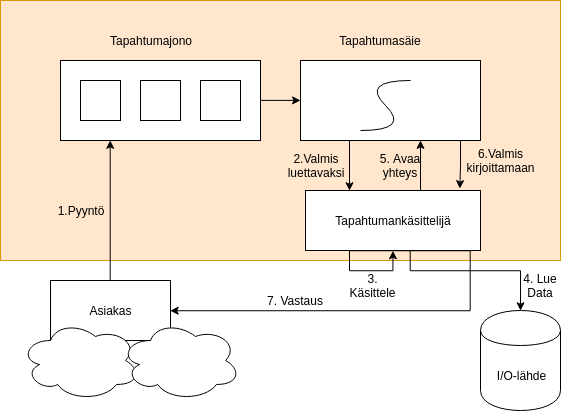
\includegraphics[scale=0.5]{reactor.png}
  \label{fig:reactor}
\end{figure}

Mallin tapahtumakäsittelijöissä samanaikaisuuteen päästään
vain I/O:n osalta, kun käytetään asynkronisia
I/O-operaatiota.
Estäviä operaatioita tulee välttää,
sillä niiden käyttäminen laskee sovelluksen
vastaavuutta huomattavasti~\cite{schmidt_reactor:_1995}.
Asynkronisia I/O-operaatioita
voidaan suorittaa niitä tarjoavien käyttöjärjestelmä kutsujen
avulla, tai siirtämällä I/O-operaatiot toisen säikeen tehtäväksi.
Itse Reactor-malli ei ota kantaa siihen, miten asynkroninen operaatio toteutetaan.
Jos tapahtumakäsittelijässä tarvitaan pitkäkestoista laskentaa
kannattaa sitä varten luoda uusi prosessi tai säie. Tämä
prosessi tai säie saattaa pyynnön loppuun rinnakkain
tapahtumasäikeen kanssa~\cite{schmidt_reactor:_1995}.

Reactor-toteutuksissa tapahtumiksi mallinnetaaan I/O-väylien
valmiutta suorittaa luku-tai kirjoitusoperaatioita~\cite{schmidt_reactor:_1995}.
Kun I/O-väylä
vapautuu tapahtumasäie viestii tapahtumakäsittelijälle, että 
I/O-operaation voi suorittaa. Sovellus siis toisinsanoen
reagoi I/O-laitteen vapautumiseen ja tästä nimi Reactor juontuu.
Näin käyttöjärjestelmä ei aseta
verkkopalvelinsovellusta odottaa tilaan I/O-operaatioiden takia.


\subsection{Proactor}

Reactor-malli on osa Proactor-mallia.
Siinä hyödynnetään käyttöjärjestelmän asynkronisia ominaisuuksia suorittamaan
operaatiota ennen pyynnön saapumista tapahtumasäikeelle~\cite{pyarali_proactor_1997}.
Reactor-mallinen osa ohjaa tässä mallissa asynkronisten tapahtumien
valmistumistapahtumia niitä vastaaville tapahtumankäsittelijöille~\cite{pyarali_proactor_1997}.

Toisin kuin Reactor-mallinen palvelin, joka reagoi I/O-laitteen vapautumiseen,
Proactor-mallinen palvelin reagoi vasta kun, käyttäjärjestelmä
on suorittanut I/O:n asynkronisesti sen puolesta. Tästä käytetään nimitystä
proaktiivinen I/O semantiikka, josta nimi proactor juontuu ~\cite{pyarali_proactor_1997}.

Proactor mallin tavoite on yksinkertaistaa asynkronisten ohjelmien kehitystä.
Proactor-mallissa voidaan suoraviivaisesti suorittaa toisistaan riippuvaisia
asynkronisia operaatioita, asettamalla asynkronisten tapahtumien valmistumisille
käsittelijöitä.
Tätä toimintatapaa kutsutaan vastakutsuksi.
Vastakutsuja voi asettaa sisäkkäin ja näin voidaan rakentaa riippuvaisten
asynkronisten operaatioden ketjuja. Ketjuilla voidaan
rakentaa peräkkäistä I/O-logiikkaa estämättä muiden asiakkaiden
pyyntöjen käsittelyä.

Proactor-mallia suositellaan käytettäväksi, jos sovellus vaatii
asynkronisten operaatioiden kutsumista ja sovellus tarvitsee ilmoituksen
asynkronisen operaation valmistumisesta.
Pyyntöjen käsittely Proactor-mallissa käydään läpi kuvassa~\ref{fig:proactor}.
Kuva~\ref{fig:proactor} noudattaa Proactorin~\cite{pyarali_proactor_1997} esittelyyn tehtyä
kuvaa, jossa Proactor-palvelin käsittelee pyynnön, mutta kuvassa~\ref{fig:proactor}
korostetaan Proactoriin-sisältyvää Reactor-mallia.
\begin{figure}
  \caption{Pyynnön käsittely Proactor-mallissa~\cite{pyarali_proactor_1997}}
  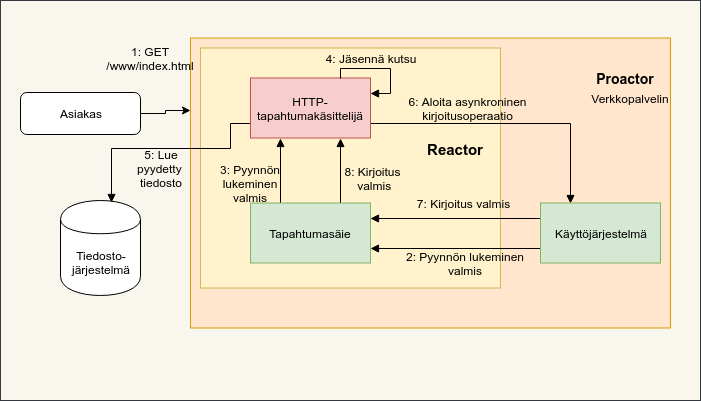
\includegraphics[scale=0.5]{Proactor.png}
  \label{fig:proactor}
\end{figure}
Pyynnön käsittely Proactor-mallisessa palvelimessa~\cite{pyarali_proactor_1997} 
tapahtuu seuraavasti:
    \begin{enumerate}
      \item Asiakas lähettää HTTP GET pyynnön.
      \item Käyttöjärjestelmä lukee pyyntöä sovittuun puskuriin ja ilmoittaa kun valmis.
      \item Valmistumisohjaaja (Reactor) kutsuu HTTP-tapahtumakäsittelijää.
        Kohdat 2 ja 3 toistuu kunnes koko pyyntö on luettu.
      \item HTTP-tapahtumakäsittelijä jäsentää kutsun. Eli
        käytännössä selvittää minkä tiedoston asiakas haluaa.
      \item HTTP-tapahtumakäsittelijä lukee pyydetyn tiedoston.
      \item HTTP-tapahtumankäsittelijä aloittaa asynkronisen operaation
        kirjoittaakseen tiedoston datan asiakasyhteyteen, ja asettaa
        itsensä tapahtumakäsittelijäksi kirjoituksen valmistumiselle.
      \item Kun kirjoitusoperaatio on valmis käyttöjärjestelmä ilmoittaa
        Valmistumisohjaajalle.
      \item Valmistumisohjaaja huomauttaa HTTP-tapahtumakäsittelijää,
        koska se asetti itsensä tapahtumankäsittelijäksi kirjoituksen
        valmistumiselle. Kohtia 6 - 8 toistetaan kunnes koko tiedosto on lähetetty.
    \end{enumerate}
Niin kuin Reactor-malli, Proactor ei myöskään sovellu laskennan rinnakkaistamiseen.
Proactorin muutokset rajoittuvat asynkronisten-operaatioden ohjaamisen
kehittämiseen. Mallissa tapahtumasäie kutsuu tapahtumankäsittelijöitä, jolloin
pitkäkestoisen laskennan suorittaminen tapahtumankäsittelijässä, johtaisi
muiden pyyntöjen odotusajan kasvuun. Malliin pitää siis
lisätä muita mekanismeja laskennan rinnakkaistamiseksi.
% TODO: lisää proactor-paperissa esitettyjä mekanismeja

Modernissa verkkopalvelinsovelluksessa Proactor-mallin suosioon on
monta syytä. RESTful-rajapinnan käyttäminen
verkkopalvelinsovelluksessa viestien välitykseen,
saa viestien koon pysymään pienenä ja viestien
käsittelyyn kuluvan ajan lyhyempänä verrattuna
HTML-tiedosto vastaukseen[lähde?]. % Etsi joku REST-lähde
Monisäikeisyys ja rinnakkaistaminen
voidaan järjestelmän arkkitehtuurissa siirtää tietokantamoottorin vastuulle,
jolloin verkkopalvelin voi lähettää sille asynkronisia kyselyitä
ja näin suorittaa useisiin pyyntöihin liittyviä tietokantakyselyitä
samanaikaisesti. Tämä vaatii Proactor-mallin sillä asynkronisen tietokantaoperaatioon
pitää kytkeä vastakutsu tiedon käsittelyyn ja lähettämiseen.
Tämänkaltaisella toteutuksella verkkopalvelimen käyttötapaus sopii
hyvin yhteen Proactor-mallin määrittelyn kanssa tukeutuen
mallin vahvuuksiin sekä peittäen sen heikkouksia.

\subsection{AMPED}

AMPED on asynkroninen tapahtumaohjattu malli, jossa
tapahtumasäie suorittaa suurimman osan prosessoinnista. 
Sen erikoispiirre on, että estävät I/O-kutsut
siiretään apulaisten vastuulle, jolloin
ne ei estä tapahtumasäiettä. Apulaiset voivat
olla joko prosesseja tai ytimentasonsäikeitä.
Tällä mekaninsmilla muutetaan käyttöjärjestelmän
estävät pyynnöt tapahtumasäikeen näkökulmasta
asynkronisiksi.

% TODO: Siirrä kaikkien mallien jälkeen ja lisää suhde säiereserviin
% TODO: Onko libuv enää oleellista
Tässä tutkielmassa keskitytään erityisesti
Proactor-malliin, sillä se on sisäänrakennettu Node.js ohjelmaympäristöön ja
täten paljon käytetty. Node.js:n Proactor-mallin toteuttamisesta vastaa
libuv-kirjasto~\cite{libuv_design_2019}. Suunnittelufilosofiassa
libuv:lla on paljon yhteistä AMPED-mallin kanssa, sillä
sen tarkoitus on taata aina asynkroniset I/O-operaatiot alustasta
riippumatta. Libuv siirtääkin I/O-kutsun toiselle säikeelle
jos alustalla ei ole tarjota asynkronista kutsua~\cite{libuv_design_2019}.
Tämä toimintapa saa kutsun näyttämään tapahtumankäsittelijästä
asynkroniselta.

\subsection{SEDA ja SYMPED}

Toinen Reactor mallin laajennus on SEDA (Staged Event Driven Architecture)~\cite{welsh_seda_2001}.
Siinä pyyntöjen käsittely jaetaan tasoiksi, joissa kaikissa on
käytännössä reactor-mallin toteuttava rakenne. Jokaisella tasolla
on oma tapahtumajono sekä tapahtumakäsittelijä, joka ohjaa työtä
apusäikeille. Tasoilla ei ole tapahtumasäiettä, sillä
jokaisella tasolla on vain yksi tapahtumakäsittelijä.
Tapahtumakäsittelijä voi käsittelyn päätteeksi
lisätä uusia tapahtumia seuraavien tasojen tapahtumajonoihin.
Tämän lisäksi jokaisella tasolla on resurssiohjaaja,
joka vastaa resurssien käytön pysymisestä sallitulla tasolla,
sekä apusäikeiden määrästä kyseisellä tasolla~\cite{welsh_seda_2001}.
SEDA-arkkitehtuurin suurin ero suoraan Reactor-mallin pohjalta luotuun
palvelimeen on sen hienojakoisempi resurssien ohjaus sovelluksen eri tasoille.
SEDA-arkkitehtuurilla on mahdollista myös saavuttaa rinnakkaisuutta
laskennallisesti vaativissa tehtävissä.

Reactor-mallia voi laajentaa vielä kolmannella tavalla.
Jos samaa Reactor-sovellusta ajaa yhdessä eri säikeillä tai prosesseilla
ja jokin säie jakaa työn tasaisesti tapahtumasäikeiden välillä
on kyseessä SYMPED-malli. Näin Reactor-toteutuksen
skaalautuvuutta voidaan jälkikäteen parantaa.

\section{Mallien vertailu ja analyysi}\label{sec:vertailu}
Seuraavaksi esitellään arviointikriteerit,
joilla malleja vertaillaan.
Vertailu perustuu aiempaan kirjallisuuteen, niissä
tehtyihin testeihin ja arvioihin
mallien soveltuvuudesta eri
käyttötapauksiin.
Vertailua ohjaava ajatus on:
edistääkö mallin käyttäminen palvelimen
suorituskykyä rinnakkaisuutta kasvattamalla
nostamatta sovelluslogiikan kehitystyön haastavuutta
sietämättömälle tasolle.

\subsection{Arviontikriteerit}

Palvelimen roolin kannalta olisi toivottavaa, että
se pystyisi käsittelemään mahdollisimman paljon pyyntöjä
ajan yksikössä. Pyyntöjen volyymia voidaan
mitata täytettyjen pyyntöjen määrällä ajan suhteen.

Sen tulisi pystyä myös käsittelemään pyyntöjä
luotettavasti eli lopulta kaikki pyynnöt käsitellään ja niihin vastataan.

Yksittäiselle asiakkaalle tärkein suorituskyvyn mittari on se kuinka kauan
yksittäiseen pyyntöön vastaaminen vie.
Pyynnön pieni viive saa
palvelun käyttökokemuksen tuntumaan sujuvammalta.
Viivettä mitataan millisekunteina.
Pyyntöjen keskimääräinen viive ja käsiteltyjen pyyntöjen
volyymi ovat kääntäen verrannollisia.

Skaalautuvuus on tärkeää palvelinta ylläpitävälle taholle, sillä
näin käyttäjämäärän kasvaessa voidaan suorituskykyä parantaa
lisäämällä laitteistoresursseja. Skaalautuvuutta voidaan
mitata ajamalla toteutuksia eri tehoisilla laitteistoilla
ja vertailemalla kuinka paljon suorituskyky muuttuu 
parantuneiden laitteistoresussien myötä.

Verkkopalvelinsovelluksen tulisi
olla vakaa. Vakauden määrittää
se todennäköisyys, joka sovelluksella on
päätyä kriittiseen virhetilanteeseen. Kriittisessä
virhetilanteessa sovellus ei osaa
itse palautua sellaiseen tilaan, jossa
toiminta voisi jatkua normaalisti ja oikein.
Virhetilaan voidaan päätyä käytännössä
ohjelmointivirheen, laitteistovirheen tai hyökkäyksen seurauksena.
Verkkopalvelinsovelluksen samanaikaistamismalli
vaikuttaa etenkin ohjelmointivirheiden todennäköisyyteen,
ja voi tehdä tietyistä hyökkäyksistä lamauttavampia.


Verkkopalvelimen samanaikaistamiskäytännön tulisi
yksinkertaistaa samanaikaisuuden hallintaa sovelluksessa~\cite{pyarali_proactor_1997}.

Kehitystyön helpottaminen vähentää kustannuksia
järjestelmän, kun järjestelmää rakennetaan, laajennetaan ja ylläpidetään.
Siksi järjestelmän rakenteen yksinkertaisuus ja
ymmärrettävyys on haluttava ominaisuus.

Näin on valittu seuraavat kriteerit
järjestelmien vertailuun.
\begin{itemize}
  \item käsiteltyjen pyyntöjen määrä eli volyymi
  \item menetysprosentti
  \item skaalautuvuus laitteistoresursseihin
  \item viive
  \item vakaus
  \item kehitystyön haastavuus
\end{itemize}

\subsection{Järjestelmien volyymin ja skaalautuvuuden testit simulaatiolla}
Vuonna 1997 James C. Hu et.al testeissään~\cite{hu_measuring_1997} huomasivat
että pienillä tiedostoilla säiereservimalli oli paras,
mutta suuremmilla tiedostoilla Proactor-palvelin oli kaikista tehokkain.
Testissä asynkronisia operaatioita hidasti
erityisesti TransmitFile-funktio, joka oli
hidas pienillä tiedostoilla.
Proactor-toteutus käytti tätä kutsua I/O:n hallitsemiseen,
kun taas säiereservi-toteutus käytti estävää I/O:ta.

Tästä tuloksesta voidaan huomata,
että suurilla tiedostoilla asynkroniset kutsut
pitävät I/O-resurssien käyttöasteen hyvin suurena.
Käyttöjärjestelmä pystyy siis tehokkaasti hallitsemaan
suurten asynkronisten operaatioiden aikataulutusta
I/O-laitteilla.

TransmitFile-funktio aiheutti pienillä 500-tavuisilla tiedostoilla hyvin suuren viiveen
vastauksille, joka oli noin 200 ms. Samalla tiedostokoolla säiereservimallin palvelin
suoriutui vain noin 50 ms viiveellä.
50 K kokoisilla tiedostoilla proactor
palvelimen viive laski alle säiereservimallin arvon.
Suuremmilla tiedostoilla
ero korostui entisestään.
Pienillä tiedostoilla säiereservimallilla oli suurempi
volyymi, mutta myös tämä tilanne kääntyi tiedostokoon kasvaessa.

Pohdittavaksi jää miten uudemmat käyttöjärjestelmissä
toteutetut asynkroniset kutsut suoriutuisivat 
vastaavassa kokeessa.

Ivan Voras ja Mario Zagar testasivat~\cite{voras_characteristics_2009},
palvelimen rinnakkaistamismalleja mdcached keskusmuistitietokantaan.
Testissä oli mukana SPED eli reactor-toteutus, SEDA-toteutus ja AMPED-toteutus.
Keskusmuistitietokannan erikoispiirre on että, siihen ei liity lainkaan levy I/O:ta
vaan toteutuksen suorituskyky on pääasiassa riippuvainen muistiväylän nopeudesta sekä
käyttöjärjestelmäkutsujen nopeudesta. Tämä eroaa tavanomaisesta
verkkopalvelin sovelluksesta, jossa usein tarvitaan levy-I/O:ta 
eri tiedostojen lukemiseen.

Toteutuksista mitattiin operaatioiden (transaction) määrä sekunnissa vaihtuvilla tietyillä
asiakasmäärillä. Kaikki mallit testattiin samalla laitteistolla.

Testissä he huomasivat,
että heidän SEDA-toteutuksensa kahdella tapahtumasäikeellä ja 4 apusäikeellä
ei saavuttanut huomattavaa
etua yksinkertaiseen Reactor-toteutukseen. Tämän diagnosoitiin
johtuvan SEDA:n aiheuttamien suoritinympäristön vaihtojen yleisyydestä
sekä säikeiden välisestä kommunikoinnista.
Testissä molempien järjestelmien suorituskyky
oli lähes samalla 120:een asiakkaaseen asti jonka
jälkeen SPED-järjestelmän suorituskyky alkoi
hieman heikentyä. SPED suoritti silloin noin 110 000 toimitusta sekunnissa
ja SEDA 120 000 sekunnissa.

SEDA-mallissa jokaisella käsittelyn vaiheella on omat apusäikeensä,
joilla saadaan rinnakkaistettua vaiheeseen liittyvää estävää laskentaa.
Muistitietokannan käyttötapauksessa estävää laskentaa on vähäisesti.
Kuitenkin vaiheesta toiseen siirtyminen aiheuttaa suoritinympäristön vaihdon,
kun uuden vaiheen apusäie otetaan käyttöön.
Apusäikeiden hyödyt
tulisivat näkyviin selkeämmin käyttötapauksessa, jossa vaaditaan enemmän
rinnakkaista estävää laskentaa, kun Muistitietokannan tapauksessa.

Samassa testissä AMPED-järjestelmä neljällä apuprosessilla
kykeni 250 000 toimitukseen sekunnissa 120:nellä asiakkaalla. Mielenkiintoista on
että heidän SEDA-toteutus, jossa tapahtumasäikeiden ja apusäikeiden
määrät asetettiin samaksi arvoksi suoritui huomattavasti paremmin ja
saavutti 300 000 tapahtumaa sekunnissa 120:nellä asiakkaalla.
Vertailun selkein voittaja skaalautuvuuden
osalla oli SYMPED-järjestelmä, jossa on useita SPED-järjestelmiä
omilla säikeillään. Tällä järjestelmällä neljällä säikeellä
saavutettiin 440 toimitusta sekunnissa 120:nellä asiakkaalla.
SYMPED-järjestelmä osoitti myös hyvää skaalautuvuutta
sille annettujen säikeiden määrän kasvaessa.


\subsection{Sovelluslogiikan kehitystyön haastavuus}
Rinnakkaistamisen toteutusmallit ovat työkaluja kehittäjälle,
jotka toteutetaan mielekkäästi kirjastona tai moduulina.
Jos malli on hyvin toteutettu kehittäjän tulisi pystyä
keskittymään keskeisen sovelluslogiikan kirjoittamiseen
murehtimatta rinnakkaisuutta hallitsevasta osasta.

Reactor-malli on yksinkertainen ja helpommin toteutettava
kuin Proactor. Reactor-mallin onnistuu hyvin tavoitteessaan
erottaa pyyntöjen samanaikaistamiseen liittyvä logiikka
muusta sovelluslogiikasta.
Tapahtumaohjatut sovellukset tuovat omat haasteensa
kehittäjälle, sillä niistä virheiden löytäminen ja
korjaaminen on usein työlästä, koska ohjelman
suoritus ei kulje rivi riviltä, vaan järjestys
muuttuu tapahtumakäsittelijöiden ja vastakutsujen mukaan.

Reactor-mallia käyttävässä palvelimessa kehittäjän
pitää huolehtia siitä, että yksittäisen pyynnön
käsittelyyn menee vähän aikaa~\cite{pyarali_proactor_1997}, koska
tapahtumasäikeen aika pitää jakaa tehokkaasti
kaikkien pyyntöjen välillä. Tämä saavutetaan
vain vähälogiikkaisilla tapahtumankäsittelijöillä, sekä
asynkronisilla I/O-kutsuilla.

Reactor-mallin toteutuksissa kehittäjän tulee huomioida
asynkronisen I/O:n vaikutukset. Asynkronisuus vaikeuttaa koodin
luettavuutta, mutta se nostaa ohjelman samanaikaisuutta ja täten
tehokkuutta huomattavasti. Sovelluslogiikan kehittäjän
tulee myös huolehtia, että kirjoitettava logiikka
käyttää asynkronisia kutsuja~\cite{pyarali_proactor_1997}, sillä estävät
kutsut pysäyttävät koko sovelluksen suorituksen.

Ongelmana on myös pidetty käyttöjärjestelmien huonoa
tukea asynkronisille kutsuille~\cite{pyarali_proactor_1997}. Järjestelmäkutsu
$select$ johon, perustui käyttöjärjestelmien Reactor-toteutuksia,
ei salli useamman säikeen odottaa saman tunnistejoukon tapahtumia.
Tämä ominaisuus estää tehokkaan laitteiston rinnakkaisuuden hyödyntämisen.
Asynkronisten kutsujen tuki on kuitenkin parantunut.
Linux-ytimen versiossa
2.4.44 siihen lisättiin $epoll$ järjestelmäkutsu~\cite{man_epoll}, joka
sallii tapahtumapohjaisen I/O:n useammalla säikeellä
samaan aikaan. BSD-ytimessä vastaava toiminnallisuus on toteutettu $kqueue$
kutsuun.
% Yritä löytää onko kutsujen ominaisuudet muuttuneet parissa kymmenessä vuodessa
Jos ohjelman tulee käsitellä
asynkronisen operaation tulosta, tulee operaation valmistumiselle
asettaa tapahtumakäsittelijä. Tätä toimintatapaa kutsutaan vastakutsuksi (callback)
Tässä tilanteessa Proactor-malli on erittäin hyödyllinen, sillä se
kuvailee selkeästi miten asynkronisten tapahtumien valmistumisia tulisi käsitellä.

Proactor-mallissa kuten Reactor-mallissa sovelluslogiikka ohjelmoidaan
tapahtumankäsittelijöihin, mutta Proactor-mallissa liittyy
mallille tyypillisesti vastakutsuja. Jos vastakutsuja ei tarvita
voidaan vain käyttää Reactor-mallia ja olla käyttämättä Proactor-rakennetta kokonaan.
Vastakutsut ovat haastava konsepti. Ne vaikeuttavat vianetsimistä
sovelluksesta, koska sovelluksen kulku vaihtelee kehysinfrastruktuurin
ja tapahtumakäsittelijöiden logiikan välillä. Täten sovelluksen
kulkua on vaikea seurata askel askeleelta.

Vastakutsujen abstraktioita ohjelmointikielissä ovat Promise, Future ja
async/await. Ne auttavat kehittäjää hahmottamaan vastakutsujen
toimintaa korkealla tasolla.

Proactor-mallissa kehittäjän on vaikeaa vaikuttaa sovelluksen
aikataulutukseen~\cite{pyarali_proactor_1997},
sillä asynkronisten operaatioiden luojalla
ei ole mahdollisuutta ohjata operaatioiden valmistumisjärjestystä.
Toteutuksen tulisikin siksi tarjota kehittäjälle mahdollisuuden
priorisoida ja keskeyttää asynkronisia operaatioita.
Jos kehittäjä olettaa asynkronisten kutsujen valmistuvan tietyssä järjestyksessä,
voi se johtaa eräänlaiseen kilpailutilanteeseen, jossa
oikea lopputulos on riippuvainen tietystä valmistumisjärjestyksestä.
Toisistaan riippuvaisia asynkronisia operaatioita
voi suorittaa peräkkäin aiheuttamatta kilpailutilanteita ketjuttamalla ne
vastakutsuilla.

Reactor-tai Proactor-mallit eivät tarjoa keinoja
laskennan rinnakkaistamiseen. Kehittäjän tulee lisätä
mallin tapahtumakäsittelijöihin rinnakkaisuutta käsittelevää
logiikkaa kuten säikeiden luomista, silloin kun se on tarpeen.

Säiereservimallissa ohjelmakoodi voidaan pitää yksinkertaisena ja
hyvin luettavana. Kehittäjät voivat vapaasti käyttää intuitiivisia
peräkkäisiä operaatioita ja estäviä kutsuja, koska sovelluslogiikkaa
suoritetaan erillisillä säikeillä~\cite{pyarali_proactor_1997}. Estävä kutsu pysäyttää vain
sen säikeen, jonka käsittelyyn se liittyy, jolloin muiden
pyyntöjen käsittely voi jatkua esteettä.

Eri asiakkaiden pyynnöt liittyvät harvoin toisiinsa,
jolloin niiden välillä ei ole merkittävästi jaettua tilatietoa ja
synkronointia tarvitaan minimaalisesti~\cite{pyarali_proactor_1997}.
Kehittäjän tulee kuitenkin ottaa huomioon mahdolliset lukkiutumiset
tai kilpailutilanteet eri pyyntöjen välillä, jos
toteutuksessa ilmenee tarve tilatiedon jakamiselle.
Pyyntöihin liittyvä laskenta rinnakkaistuu hyvin laitteistotasolla,
kun jokainen pyyntö on käsittelyssä omalla säikeellään.

SEDA-mallissa rinnakkaisuuden hallintaa edistää
samaa tietoa käsittelevien säikeiden eristäminen samalle tasolle~\cite{welsh_seda_2001}.
Samalla tasolla synkronisoiminen ja kilpailutilanteiden ratkaiseminen on
yksinkertaisempaa kuin koko sovelluksen mittakaavassa, ja
viesteihin perustuva sovelluksen kulku on helpommin seurattavissa kuin
muissa tapahtumaohjatuissa malleissa.

% TODO: Selitä symped tarkemmin
Jos Reactor-palvelimen skaalautuvuus ei riitä palvelemaan
järjestelmän tarpeita, voidaan järjestelmän sovelluslogiikka
sovittaa suoraviivaisesti osaksi SYMPED-järjestelmää. SYMPED-toteutus
voidaan rakentaa reactor eli SPED toteutuksen ympärille. Tämä
tekee SYMPED-toteutuksesta mielekkään jatkosuunnitelman kehittäjälle,
jonka huolet skaalautuvuudesta koskavat pääasiassa palvelun tulevaisuutta.

\subsection{Vakaus}
Palvelimen vakaudella tarkoitetaan sen kykyä vastustaa hyökkäyksiä ja
virhetiloja.
Palvelimen rinnakkaisuuden toteutusmalli vaikuttaa sen vakauteen, jos asiakkaiden
pyynnöt vaikuttavat toisiinsa tai jos rinnakkaistaminen voi aiheuttaa virhetiloja kuten
lukkiutumista.

Reactor/Proactor-malliseen palvelimeen voi kohdistaa hyökkäyksiä, joilla pyritään
myrkyttämään sovelluksen tapahtumasäie. Reactor-mallin palvelin toteutuksissa
osoitepolkujen jäsentäminen on saman säikeen vastuulla kuin sovelluksen ohjaaminen.
Tämän työvaiheen takia
tapahtumasäikeen myrkyttämiseen sopivat pyynnöt,
joiden osoitepolun selvittämiseen liittyy kompleksista
säännöllisten lauseiden käsittelyä~\cite{davis_case_2017}.
Proactor-mallin kuvassa~\ref{fig:proactor} pysähdyttäisiin siis kohtaan 4: kutsun jäsentäminen, ja
kaikki muut pyynnöt joutuvat odottamaan.
Yksi pyyntö siis aiheuttaa suhteettoman suuren työtaakan
tapahtumasäikeelle, jolloin koko sovellus jää odottamaan sitä.
Hyökkääjä lähettää näitä pyyntöjä niin paljon, että sovellus
ei pysty palvelemaan sen todellisia asiakkaita. Tämä
on palvelunestohyökkäyksen erikoistapaus.

Tällaiset hyökkäykset aiheuttaisivat ongelmia myös säiereservimallia
noudattaville järjestelmille, mutta niiden pitäisi onnistua
lukitsemaan reservin jokainen säie samaan aikaan, jotta
järjestelmä ei kykenisi enää vastaamaan asiakkaiden pyyntöihin~\cite{davis_case_2017}.

Reactor-toteutukseen perustuvassa palvelinsovelluksessa ei ole
riskiä kilpailutilanteille tai lukkiutumiselle, toisin kuin säiereservimallissa.
Säiereservimallissa palvelin voi lukkiutua, jos samaan aikaan käsittelyssä olevat
pyynnöt tarvitsevat samoja resursseja käsittelyn aikana. Tämä riski on otettava
huomioon järjestelmän suunnittelussa ja sovelluslogiikan kirjoittamisessa.

Säiereservimallissa kilpailutilanteiden riski on hyvin pieni, jos pyyntöjen
välillä ei ole jaettua tilatietoa. Jaetun tilatiedon kanssa voi tulla
sivuvaikutuksia, jos pyynnöillä on mahdollisuus muokata tilatiedon sisältöä.

\subsection{Johtopäätökset}
% TODO: Lisää lähteitä johtopäätöksiin
% TODO: Erityisesti cluster-dokumentaatio
Reactor-malli erottaa
selkeästi pyyntöjen käsittelyn
samanaikaistamiseen liittyvän
logiikan muusta sovelluskohtaisesta logiikasta.
Malli on myös suhteessa muihin samanaikaisuutta
käsitteleviin malleihin yksinkertainen.
Näistä syistä se on toteutettu useisiin
kirjastoihin ja saavuttanut vakaan suosion.

Reactor-mallin rajallisuudet rinnakkaisuudessa
eivät ole haitaksi, jos järjestelmässä on rinnakkaisuutta
korkeammalla tasolla. Eli
jos Reactor-mallisia palvelmia ajetaan useita rinnakkain
ja näin luodaan SYMPED-järjestelmä.

Proactor-malli laajentaa Reactor-mallia merkittävällä tavalla,
sillä sen avulla voidaan ketjuttaa asynkronisia
operaatioita vastakutsuilla. Tämä ominaisuus
tuo joustavuutta samanaikaisen sovelluslogiikan kehittämiseen.

Proactor-mallin ansiosta rinnakkaisuus
voidaan toteuttaa myös järjestelmässä alemmalla
tasolla kuten tietokantaohjelmassa.
Proactor-palvelin voi odottaa useita asynkronisia
tietokantakyselyita samalla kun, se suorittaa
muuta logiikkaa. Eli tietokantakyselyn valmistumiskäsittelijäksi
asetetaan toiminto, joka kirjoittaa vastauksen
halutussa muodossa asiakkaalle.
Todellisen rinnakkaisen työn
suorittaa tässä käyttötapauksessa tietokantaohjelma.

Proactor-malli ei paikkaa
Reactor-mallin rajallisuutta laskennan rinnakkaistamisessa,
sillä tapahtumakäsittelijöiden logiikka suoritetaan
samalla säikeellä kuin sovelluksen kulun ohjaus.
Laskennan rinnakkaistamiseksi tapahtumakäsittelijöihin
tulee lisätä säikeiden käsittelyyn liittyvää logiikkaa.
Malli ei siis vähennä laskennan rinnakkaistamiseen liittyviä
haasteita, mutta on tehokas tapahtumien ja asynkronisten
operaatioiden hallinnassa. Nämä ominaisuudet riittävät
I/O-resurssien tehokkaaseen hyödyntämiseen.

Reactor/Proactor-mallin toteuttavalla
kirjastolla voidaan kustannustehokkaasti
toteuttaa palvelin, joka kykenee suoriutumaan
tehtävistään palvelun alkutaipaleella. Jos
käyttäjämäärät kasvavat ja skaalautuvuutta
vaaditaan voidaan järjestelmä muuttaa SYMPED-järjestelmäksi,
joka todetusti skaalautuu hyvin resursseihin.
Node.js sovelluksesta voi luoda SYMPED järjestelmän
cluster-kirjastolla.

Jos laskennan suorittaminen rinnakkain usealla suorittimella
on ainoa väylä riittävän suorituskyvyn saavuttamiseksi,
ovat säiereservimalli ja SEDA-malli parempia vaihtoehtoja.
Proactor palvelimien tapahtumakäsittelijöihin
voidaan ohjelmoida säikeiden käsittelyä, mutta tämä
on täysin soveluslogiikan kehittäjän vastuulla.
Tämänkaltainen menettely olisi hybridi
SEDA-mallin ja Proactor-mallin välillä, jossa
tapahtumankäsittelijällä on säiereservi, mutta tapahtumakäsittelijät
eivät välttämättä muodosta selvää tasohierarkiaa.

\section{Yhteenveto}\label{sec:yhteenveto}

Verkkopalvelimen voi esittää luontevasti
tapahtumaohjattuna mallina. Reactor-malli esittää yksinkertaisen
ratkaisun useista lähteistä tulevien tapahtumien käsittelyyn.

Verkkopalvelimen yleisimmät tehtävät ovat
HTML-tiedostojen ja nykyään kasvavissa määrin
tekstimuotoisen datan lähettäminen.
Näiden tehtävien suorituskyky on
I/O-sidonnainen.
Asynkronisilla luku-ja kirjoitusoperaatioilla samanaikaisuuden hallinta
voidaan siirtää käyttöjärjestelmän vastuulle, jolloin
verkkopalvelimen tehtävien täyttämiseen Proactor-mallinen
palvelin sopii hyvin.
Se esittää sopivat laajennukset Reactor-malliin, joilla
asynkronisia operaatioita voidaan hallita joustavasti.
Sillä voidaan suorittaa muista operaatioista riippuvaisia I/O-operaatioita
samanaikaisesti, ketjuttamalla niitä takaisinkutsuilla.
Asynkronisilla operaatioilla saavutetaan suuri I/O-resurssien
käyttöaste.

Jos palvelimen tarkoitus on suorittaa enemmän laskentaa kuin
I/O-operaatioita, ei Reactor-pohjainen vaihtoehto ole paras mahdollinen.
Laskentariippuvaisessa käyttötapauksessa säiereservi tai SEDA-arkkitehtuuria
noudattava toteutus takaa huomattavasti paremman suorituskyvyn kuin
Reactor-mallia noudattava.

Proactor-tai Reactor-palvelimen voi laajentaa
usean prosessin toteutukseksi, jos skaalautuvuus
yhdellä prosessilla ei ole riittävä palvelun tarpeisiin.


\bibliographystyle{plain}
\bibliography{kandi_zot}


\end{document}
